
\chapter{Implementación de ClamAV}
% \section{Herramientas de seguridad en  \emph{hardware} y \emph{software}}

\section{Instalación en el sistema  huesped}

Antes  implementar el sistema de antivirus dentro de la tarejeta de desarrollo 
\emph{XUPV2}, fue necesario conocer y manejar  el sistema dentro de una 
arquitectura x86-64 (sistema  husped).

\subsection{Requerimientos de instalación}

Para la compilaci\'on e instalci\'on del antivirus ClamAV en platafomas  
basadas en \emph{UNIX} son requeridos los siguintes componentes:

\begin{itemize}

\item Biblioteca  zlib y zlib-devel. Es una biblioteca de compresión que 
proporciona compresión en la memoria y funciones de descompresión, como 
comprobaciones de integridad de los datos sin comprimir.

La compresión se puede hacer en un solo paso si la memoria intermedias son lo 
suficientemente grandes, o puede hacerse mediante llamadas repetidas de la 
función de compresión\cite{zlib}.


\item Compilador GCC. GCC es una distribución integrada de compiladores para 
varios lenguajes de programación . Estos lenguajes actualmente incluyen C, C + 
+, Objective-C, Objective-C + +, Java, Fortran, Ada, y Go.

La  abreviatura GCC tiene varios significados en el uso común. El actual 
significado oficial es \emph{``GNU Compiler Collection''}, que se refiere 
genéricamente a la suite completa de herramientas.

El nombre históricamente significaba \emph{``GNU C Compiler''}, y este uso es 
todavía común cuando el énfasis está en la compilación de programas en 
C\cite{gcc}.

\item Biblioteca bzip y bzip-devel. La biblioteca bzip comprime archivos 
usando el algoritmo de Burrows-Wheeler\footnote{BWT, acrónimo de 
\emph {Burrows–Wheeler transform}, también conocida como compresión por 
ordenación de bloques, es un algoritmo usado en técnicas de compresión de 
datos. } y codificación de Huffman \footnote{Codificación Huffman, es un 
algoritmo usado para compresión de datos. El término se refiere al uso de una 
tabla de códigos de longitud variable para codificar un determinado símbolo, 
donde la tabla ha sido rellenada de una manera específica basándose en la 
probabilidad estimada de aparición de cada posible valor de dicho símbolo.}.

\end{itemize}

\subsection{Instalación desde  el gestor  de paquetes del sistema  
huesped}

A continuaci\'on de  muestra como instalar  ClamAV en la arquitectura huesped:

\begin{itemize}
 \item Debian:
  \begin{verbatim}
   # apt-get update
   # apt-get install clamav
  \end{verbatim}

\end{itemize}

Estos comandos instalar\'an los siguientes paquetes: \textbf{clamav, 
clamav-base, clamav-freshclam, libbz2-1.0, libclamav1, libcurl3, libgmp3 
libidn11, ucf}

El paquete clamav-update nos crea una cron que se ejecutará cada tres horas para 
actualizar la base de datos del antivirus. Pero podemos ejecutarlo manualmente 
de la siguiente forma:

\begin{verbatim}
Proyecto@debian$ freshclam -v
Current working dir is /var/lib/clamav
Max retries == 3
ClamAV update process started at Sun May 26 13:32:16 2013
Using IPv6 aware code
Querying current.cvd.clamav.net
WARNING: Can't query current.cvd.clamav.net
WARNING: Invalid DNS reply. Falling back to HTTP mode.
Retrieving http://db.us.clamav.net/main.cvd
Trying to download http://db.us.clamav.net/main.cvd (IP: 64.22.33.90)
Downloading main.cvd [100%]
Loading signatures from main.cvd
Properly loaded 1044387 signatures from new main.cvd
main.cvd updated (version: 54, sigs: 1044387, f-level: 60, builder: sven)
Querying main.54.69.1.0.64.22.33.90.ping.clamav.net
Retrieving http://db.us.clamav.net/daily.cvd
Trying to download http://db.us.clamav.net/daily.cvd (IP: 64.22.33.90)
Downloading daily.cvd [100%]
Loading signatures from daily.cvd
Properly loaded 1298099 signatures from new daily.cvd
daily.cvd updated (version: 17271, sigs: 1298099, f-level: 63, builder: guitar)
Querying daily.17271.69.1.0.64.22.33.90.ping.clamav.net
Retrieving http://db.us.clamav.net/bytecode.cvd
Trying to download http://db.us.clamav.net/bytecode.cvd (IP: 64.22.33.90)
Downloading bytecode.cvd [100%]
Loading signatures from bytecode.cvd
Properly loaded 41 signatures from new bytecode.cvd
bytecode.cvd updated (version: 214, sigs: 41, f-level: 63, builder: neo)
Querying bytecode.214.69.1.0.64.22.33.90.ping.clamav.net
Database updated (2342527 signatures) from db.us.clamav.net (IP: 64.22.33.90)

\end{verbatim}

La configuraci\'on de ClamAV se encuentra en el archivo freshclam.conf que se 
muestra en  el \emph{Apéndice B}.

\subsection{Actualizaci\'on de firmas de virus en  ClamAV automáticamente}

Es siguiente script permite la actualizaci\'on de firmas de  manera automática 
en entornos \emph{``GNU/Linux''}


\lstinputlisting[caption=Archivo freshclam.sh,language=sh]
{./code/freshclam.sh}



\subsection{Uso de ClamAV}

Para escanear un fichero, el comando es ``clamscan'' y le indicamos el fichero:

\begin{verbatim}
Proyecto@debian$ clamscan system.ace 
system.ace: OK

----------- SCAN SUMMARY -----------
Known viruses: 2337113
Engine version: 0.97.8
Scanned directories: 0
Scanned files: 1
Infected files: 0
Data scanned: 13.55 MB
Data read: 13.48 MB (ratio 1.00:1)
Time: 5.464 sec (0 m 5 s)
Proyecto@debian$
\end{verbatim}

Para el escaneo de un directorio y todo su contenido, de manera recursiva, se 
utiliza el comando clamscan con la opción ``--r''.

\begin{verbatim}
Proyecto@debian$ clamscan -r XUPV2P-MicheAngelo/
----------- SCAN SUMMARY -----------
Known viruses: 2337113
Engine version: 0.97.8
Scanned directories: 85
Scanned files: 464
Infected files: 0
Data scanned: 163.50 MB
Data read: 238.35 MB (ratio 0.69:1)
Time: 10.768 sec (0 m 10 s)
Proyecto@debian$ clamscan -r XUPV2P-MicheAngelo/

\end{verbatim}

Para especificar que los archivos infectados solo sean movidos a un directorio 
de cuarentena, se utiliza el comando ``clamscan'' con la opción ``--move'' 
especificando un directorio que servirá como cuarentena. El directorio de 
cuarentena debe de existir previamente.

\begin{verbatim}
 Proyecto@debian$ clamscan --move=/home/Proyecto/Dropbox/UAM/PT/PT/Cuarentena/ 
/home/Proyecto/Dropbox/UAM/PT/PT/XUPV2P-MicheAngelo/
----------- SCAN SUMMARY -----------
Known viruses: 2337113
Engine version: 0.97.8
Scanned directories: 1
Scanned files: 30
Infected files: 0
Data scanned: 96.61 MB
Data read: 95.63 MB (ratio 1.01:1)
Time: 7.432 sec (0 m 7 s)
Proyecto@debian$ 
\end{verbatim}

Para especificar que los archivos infectados sean eliminados, se utiliza la 
opción ``--remove'' con el valor yes. Esta opción debe ser utilizada con 
precaución.

\begin{verbatim}
Proyecto@debian$ clamscan 
--remove=yes /home/Proyecto/Dropbox/UAM/PT/PT/XUPV2P-MicheAngelo/
----------- SCAN SUMMARY -----------
Known viruses: 2337113
Engine version: 0.97.8
Scanned directories: 1
Scanned files: 30
Infected files: 0
Data scanned: 96.61 MB
Data read: 95.63 MB (ratio 1.01:1)
Time: 7.432 sec (0 m 7 s)
Proyecto@debian$
\end{verbatim}

La salida del comando ``clamscan'' puede llegar a ser muy extensa. Si se 
desea que solo se muestre la información de los archivos infectados, se utiliza 
el comando clamscan con la opción ``--infected''.

\begin{verbatim}
Proyecto@debian$  clamscan --infected --remove=yes -r 
/home/Proyecto/Dropbox/UAM/PT/PT/XUPV2P-MicheAngelo/
----------- SCAN SUMMARY -----------
Known viruses: 2337113
Engine version: 0.97.8
Scanned directories: 85
Scanned files: 464
Infected files: 0
Data scanned: 163.50 MB
Data read: 238.35 MB (ratio 0.69:1)
Time: 10.779 sec (0 m 10 s)

\end{verbatim}

Para que el comando clamscan guarde la información de su actividad a fin de 
poder examinar posteriormente ésta a detalle, se puede utilizar éste con la 
opción ``--log'' especificando la ruta de un archivo donde se almacenará la 
bitácora de actividad.

\begin{verbatim}
Proyecto@debian$  clamscan --log=/home/Proyecto/clamscan.log  --infected 
--remove=yes -r 
/home/Proyecto/Dropbox/UAM/PT/PT/XUPV2P-MicheAngelo/


\end{verbatim}

El archivo tendr\'a el siguiente contenido:

\begin{verbatim}

----------- SCAN SUMMARY -----------
Known viruses: 2337113
Engine version: 0.97.8
Scanned directories: 85
Scanned files: 464
Infected files: 0
Data scanned: 163.50 MB
Data read: 238.35 MB (ratio 0.69:1)
Time: 10.779 sec (0 m 10 s)

\end{verbatim}


\subsection{Pruebas con ClamAV}

Por razones de seguridad no es aceptable que se envíen  virus reales para 
fines de prueba o demostración, es necesario un archivo que con seguridad 
pueda ser detectado para que el \emph{software} antivirus reaccione como 
si fuera un virus.

Existe un archivo de prueba de este tipo. Varios investigadores de antivirus ya 
han trabajado juntos para producir un archivo que  los antivirus 
``detecten'', como si se tratara de un virus.

Acordar un archivo para tales fines simplifica las cosas para los usuarios: en 
el pasado, la mayoría de los vendedores tenían sus propios archivos de prueba 
pseudo-virales que su producto sería reaccionar, pero que otros productos 
ignoraría.

\subsubsection{Archivo de pruebaAnti-\emph{Malware}}

El archivo ``eicar.com'' es un archivo DOS que consiste de caracteres ASCII con 
68 bytes de longitud.

\begin{verbatim}
 X5O!P%@AP[4\PZX54(P^)7CC)7}$EICAR-STANDARD-ANTIVIRUS-TEST-FILE!$H+H*
\end{verbatim}

\begin{verbatim}
Proyecto@debian$ cat eicar.com && clamscan eicar.com 
X5O!P%@AP[4\PZX54(P^)7CC)7}$EICAR-STANDARD-ANTIVIRUS-TEST-FILE!$H+H*
eicar.com: Eicar-Test-Signature FOUND

----------- SCAN SUMMARY -----------
Known viruses: 2337113
Engine version: 0.97.8
Scanned directories: 0
Scanned files: 1
Infected files: 1
Data scanned: 0.00 MB
Data read: 0.00 MB (ratio 0.00:1)
Time: 4.861 sec (0 m 4 s)
\end{verbatim}

\section{Instalación desde los archivos fuente en el sistema  huesped}

Para instalar la \'ultima  versi\'on de ClamAV desde las fuentes se debe de 
seguir el siguiente proceso:

\begin{itemize}
 \item Descargar la \'ultima  versi\'on disponible de ClamAV:
 \begin{verbatim}
 Proyecto@debian$ wget 
 http://downloads.sourceforge.net/clamav/clamav-0.97.8.tar.gz
 \end{verbatim}
 \item Se procede descomprimir el archivo fuente  ya  a crear  un   grupo y un 
usuario para ClamAV:
 \begin{verbatim}
  Proyecto@debian$ tar xzf clamav-0.97.8.tar.gz
  Proyecto@debian$ adduser clamav --no-create-home --disabled-password
 \end{verbatim}
 
  \item Para poder compilar ClamAV primero se deber\'a configurar el archivo 
``.config''
 \begin{verbatim}
  Proyecto@debian$./configure --enable-experimental
 \end{verbatim}
 Con lo que se obtiene la siguiente salida:
 
 \begin{verbatim}
 configure: Summary of detected features follows
              OS          : linux-gnu
              pthreads    : yes (-lpthread)
configure: Summary of miscellaneous  features
              check       : no (auto)
              clamuko     : yes
              fdpassing   : 1
              IPv6        : yes
configure: Summary of optional tools
              clamdtop    : -lncurses (auto)
              milter      : yes (disabled)
configure: Summary of engine performance features)
              release mode: yes
              jit         : yes (auto)
              mempool     : yes
configure: Summary of engine detection features
              autoit_ea06 : yes
              bzip2       : ok
              zlib        : /usr
              unrar       : yes
 \end{verbatim}

\item Se debe de comprobar que no   exista  ninguna   instalación previa en el 
sistema huesped:
\begin{verbatim}
 Proyecto@debian$ sudo make uninstall
\end{verbatim}
\item Se procede a la instalación:
\begin{verbatim}
 Proyecto@debian$ make install
\end{verbatim}
\item Para comprobar la correcta instalación de ClamAV se raliza una prueba con 
El archivo ``eicar.com''

\begin{verbatim}
 
\end{verbatim}


\end{itemize}

\section{Compilación cruzada de ClamAV desde el sistema huesped}

\subsection{Preparación del entorno de desarrollo con \emph{Buildroot}}

Se preparó un entorno de desarrollo con \emph{Buildroot}, de la misma forma 
que se  hizó para compilar las fuentes del \emph{kernel} lo cual nos permitió 
crear una \emph{toolchain} para compilar cruzadamente desde x86-64 hacía 
\emph{PowerPC} (la arquitectura objetivo).

\subsubsection{Sistema objetivo}

A continuación se muestran las  características del sistema objetivo:

  \begin{itemize}
  \item FPGA Virtex-2 Pro XC2VP30  con 30,816 celdas lógicas, 136 18-bit
multiplicadores,
  2,448Kb bloques de RAM y 2 Procesadores PowerPC.
  \item DDR SDRAM DIMM de hasta  2Gbytes de RAM
  \item Puerto Ethernet 10/100
  \item Puerto USB2 
  \item Lector de tarjetas Compact Flash
  \item Puerto de video XSGA
  \item Audio Codec
  \item Puertos SATA, S/2 y RS-232
  \end{itemize}
   
\begin{figure}[ht]
 \centering
 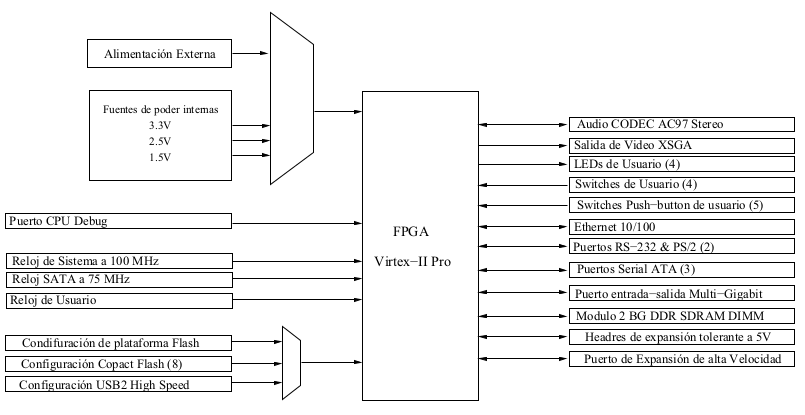
\includegraphics[scale=.50]{./figuras/virtex.png}
 % capas.png: 607x522 pixel, 72dpi, 21.41x18.41 cm, bb=0 0 607 522
 \caption{Diagrama a bloques de la tarjeta Virtex-II Pro 50}
 \label{Diagrama a bloques de la tarjeta Virtex-II Pro 50}
\end{figure}

\begin{verbatim}
#Host x86
#Creacion del directorio de trabajo y descargar buildroot
cd /opt
mkdir toolchains-mips
cd toolchains-mips
wget "http://buildroot.uclibc.org/downloads/buildroot-2011.05.tar.gz"
tar zxvf buildroot-2011.05.tar.gz
cd buildroot-2011.05
\end{verbatim}

Una de las  variables muy importantes para preparar el entorno de compilación, 
es determinar de forma correcta  la arquitectura, por se deben de verificar  
los parametros básicos de la tarejeta de desarrollo :

\begin{verbatim}
[root@XUPV2P-MicheAngelo ~]# cat /proc/cpuinfo                                  
processor       : 0                                                             
cpu             : Virtex-II Pro                                                 
clock           : 300.000000MHz                                                 
revision        : 8.160 (pvr 2001 08a0)                                         
bogomips        : 600.00                                                        
timebase        : 300000000                                                     
platform        : Xilinx Virtex                                                 
model           : testing                                                       
Memory          : 128 MB 
\end{verbatim}

Una vez que \emph{buildroot} genere la toolchain que se usará para la 
compilación de ClamAV se deberán de cambiar las variables de entorno a través 
de la ejecucion del siguiente script:


\lstinputlisting[caption=Archivo variables.sh,language=sh]
{./code/variables.sh}


Una vez  cargadas la variables de entorno de procede a preparar la instalación 
de   clamAV primero se deber\'a configurar el archivo ``.config''
\begin{verbatim}
 Proyecto@debian$./configure --enable-experimental
\end{verbatim}

Tras lo cual se obtiene la siguiente salida:
\begin{verbatim}
checking build system type... x86_64-unknown-linux-gnu
checking host system type... x86_64-unknown-linux-gnu
checking target system type... x86_64-unknown-linux-gnu
creating target.h - canonical system defines
checking for a BSD-compatible install... /usr/bin/install -c
checking whether build environment is sane... yes
checking for a thread-safe mkdir -p... /bin/mkdir -p
checking for gawk... no
checking for mawk... mawk
checking whether make sets $(MAKE)... yes
checking how to create a ustar tar archive... gnutar
checking for gawk... (cached) mawk
checking for a BSD-compatible install... /usr/bin/install -c
checking whether ln -s works... yes
checking whether make sets $(MAKE)... (cached) yes
checking for style of include used by make... GNU
checking for gcc... 
/home/Proyecto/buildroot-2013.05/output/host/usr/bin/powerpc-linux-gcc
checking for C compiler default output file name... a.out
checking whether the C compiler works... configure: error: in 
`/home/henry/buildroot-2013.05/clamav-0.97.8':
configure: error: cannot run C compiled programs.
If you meant to cross compile, use `--host'.
See `config.log' for more details.
\end{verbatim}


Este error en el archivo nos indica que  es necesario utilizar la bandera 
\emph{--host} si se requiere hacer una compilación cruzada.

Se procede nuevamente a  ejecutar el script  de autoconfiguración añadienendo 
la bandera \emph{--host} con la arquitectura objetivo:

\begin{verbatim}
 Proyecto@debian$./configure --host=ppc-unknown-linux-gnu 
--target=ppc-unknown-linux-gnu --enable-llvm CFLAGS="-O0"  --disable-nls 
--disable-libasprintf

\end{verbatim}


Una vez ejecutado el comando anterior se obtiene:

\begin{verbatim}
configure: Summary of detected features follows
              OS          : linux-gnu
              pthreads    : yes (-lpthread)
configure: Summary of miscellaneous  features
              check       : no (auto)
              fanotify    : yes
              fdpassing   : 0
              IPv6        : no
configure: Summary of optional tools
              clamdtop    : -lncurses (auto)
              milter      : yes (disabled)
configure: Summary of engine performance features)
              release mode: yes
              jit         : yes
              mempool     : no
configure: Summary of engine detection features
              autoit_ea06 : yes
              bzip2       : ok
              zlib        : /usr
              unrar       : yes
configure: WARNING:
****** WARNING:
****** You are cross compiling to a different host or you are
****** linking to bugged system libraries or you have manually
****** disabled important configure checks.
****** Please be aware that this build may be badly broken.
****** DO NOT REPORT BUGS BASED ON THIS BUILD !!!


\end{verbatim}

La salida completa del script  de autoconfiguración se muestra en el 
\emph{Apéndice B}.


Antes de continuar con el proceso de compilación es necesario desinstalar 
cualquier  verisión de ClamAV previamente instalada:

\begin{verbatim}
 Proyecto@debian$ sudo make uninstall
\end{verbatim}

Y se procede con la instalación para generar los binarios en la arquitectura 
huesped:

\begin{verbatim}
 Proyecto@debian$ sudo make
 Proyecto@debian$ sudo make install
\end{verbatim}


Debido a que se esta realizando una  compilación cruzada, es necesario depurar 
manualmente algunos de los archivos fuente.

Una vez  compilado los archivos fuente del antivirus ClamAV se debe de copiar 
la salida a los directorios correspondientes de la tarjeta a través de 
\emph{ssh} usando el comando  \emph{scp}.


El  antivirus ppuede ser probado en la tarjeta de desarrollo de la siguiente  
forma:

\begin{verbatim}
Proyecto@debian$ cat eicar.com && clamscan eicar.com 
X5O!P%@AP[4\PZX54(P^)7CC)7}$EICAR-STANDARD-ANTIVIRUS-TEST-FILE!$H+H*
eicar.com: Eicar-Test-Signature FOUND

----------- SCAN SUMMARY -----------
Known viruses: 2337113
Engine version: 0.97.8
Scanned directories: 0
Scanned files: 1
Infected files: 1
Data scanned: 0.00 MB
Data read: 0.00 MB (ratio 0.00:1)
Time: 4.861 sec (0 m 4 s)
\end{verbatim}


El archivo anterior es un archivo DOS que consiste de caracteres ASCII con 
68 bytes de longitud.

\begin{verbatim}
 X5O!P%@AP[4\PZX54(P^)7CC)7}$EICAR-STANDARD-ANTIVIRUS-TEST-FILE!$H+H*
\end{verbatim}


El antivirus  implementado  en la tarjeta deberá de  detectar esta y otras 
amenzas mientras  hace  una revisión programada ocn el comendo \emph{clamscan} 
en el sistema empotrado en la FPGA.













